\documentclass{beamer}
\setbeamertemplate{navigation symbols}{}
%\usetheme{AnnArbor}
%\usetheme{Antibes}
%\usetheme{Bergen}
%\usetheme{Berkeley}
%\usetheme{Berlin}
%\usetheme{Boadilla}
%\usetheme{boxes}
%\usetheme{CambridgeUS}
%\usetheme{Copenhagen}
%\usetheme{Darmstadt}technology
%\usetheme{default}
%\usetheme{Frankfurt}
%\usetheme{Goettingen}
%\usetheme{Hannover}
%\usetheme{Ilmenau}
%\usetheme{JuanLesPins}
%\usetheme{Luebeck}
%\usetheme{Madrid}
%\usetheme{Malmoe}
%\usetheme{Marburg}
%\usetheme{Montpellier}
%\usetheme{PaloAlto}
%\usetheme{Pittsburgh}
%\usetheme{Rochester}
%\usetheme{Singapore}
%\usetheme{Szeged}
\usetheme{Warsaw}
\usecolortheme{beaver}
\usepackage{pgfplots}

\usepackage{ragged2e}
\usepackage{algorithm2e}
\usepackage[noend]{algorithmic}
\usepackage{amsmath,amssymb}
\usefonttheme{professionalfonts}
\usepackage{helvet}
\usepackage{caption}
\usepackage[]{graphicx}
\usepackage{algorithmic}
\usepackage{multicol}
\renewcommand{\familydefault}{\sfdefault}
	
\usepackage{hanging}
\usepackage{lipsum}
\newcommand\blfootnote[1]{%
  \begingroup
  \renewcommand\thefootnote{}\footnote{#1}%
  \addtocounter{footnote}{-1}%
  \endgroup
}

\usepackage[style=authortitle,backend=bibtex]{biblatex}
\addbibresource{refer.bib}
\makeatletter
\renewcommand*{\footnoterule}{\kern -55pt \hrule \@width 2in \kern 4.6pt}
    \def\@makefnmark{\hbox{{{\usebeamercolor[fg]{footnote mark}\usebeamerfont*{footnote mark} [\@thefnmark]}}}}

    \def\@makefntext#1{%
        \def\insertfootnotetext{ #1}%
        \def\insertfootnotemark{\@makefnmark}%
        \usebeamertemplate***{footnote}}    
\makeatother
\setbeamertemplate{footnote}{\tiny \hangpara{1em}{1}\makebox[1em][l]{\insertfootnotemark}\footnotesize\insertfootnotetext\par}
\let\footnotesize\tiny
\defbeamertemplate*{footline}{shadow theme}
{%
  \leavevmode%
  \hbox{\begin{beamercolorbox}[wd=.5\paperwidth,ht=2.5ex,dp=1.125ex,leftskip=.3cm plus1fil,rightskip=.3cm]{author in head/foot}%
    \usebeamerfont{author in head/foot}\insertframenumber\,/\,\inserttotalframenumber\hfill\insertshortauthor
  \end{beamercolorbox}%
  \begin{beamercolorbox}[wd=.5\paperwidth,ht=2.5ex,dp=1.125ex,leftskip=.3cm,rightskip=.3cm plus1fil]{title in head/foot}%
    \usebeamerfont{title in head/foot}\insertshorttitle%
  \end{beamercolorbox}}%
  \vskip0pt%
}
\hyphenation{can-di-da-te}

\title[ZEMI]{Low-Density Parity Check (LDPC) Codes Design for Indonesia Digital Television DVB-T2}

\author[Citra Yasin Akbar Fadhlika]{Citra Yasin Akbar Fadhlika }
% - Give the names in the same order as the appear in the paper.
% - Use the \inst{?} command only if the authors have different
%   affiliation.

\institute[Telkom University] % (optional, but mostly needed)
{ 	Center for Advanced Wireless Technologies (AdWiTech),\\
	School of Electrical Engineering, Telkom University, Bandung\\
%	Email: \{ikhfanammar@telkomuniversity.ac.id\}
}
\date[Bandung, \today]
{ \scriptsize{\today}}
%\footnotesize{Selected Topic 1\\Mid Semester Presentation}\\ 
%March 19$\mathsf{^{th}}$, 2018}}

%\pgfdeclareimage[height=0.5cm]{university-logo}{pict/adwitech.jpg}
%\logo{\pgfuseimage{university-logo}}

%Untuk menampilkan logo
\logo{
\includegraphics[scale=0.2]{pict/telu.jpg}\vspace{232pt}\hspace{242pt}
\includegraphics[scale=0.04]{pict/adwitech.jpg}\hspace{3pt}}
%\logo{
\includegraphics[scale=0.2]{pict/telu.jpg}\vspace{-5pt}\hspace{242pt}
\includegraphics[scale=0.04]{pict/adwitech.jpg}\hspace{3pt}}
\setbeamersize{text margin left=0.5cm,text margin right=0.5cm}

\begin{document}
\begin{frame}
  \titlepage
\end{frame}
%-----------------------------------------------------------------------------------------
%bikin frame
\begin{frame}
\frametitle{Outlines}
\begin{enumerate}
%\item Introduction
\item Motivation
\item Basic Theories
\item Research Trajectory
%\item Analysis
\item Conclusion 
\end{enumerate}
\end{frame}


%\begin{frame}{Outline}
%  \tableofcontents
%  % You might wish to add the option [pausesections]
%\end{frame}

% Section and subsections will appear in the presentation overview
% and table of contents.
%\section{Motivations}
%\begin{frame}
%\tableofcontents[currentsection,currentsubsection]
%\end{frame}
%--------------------------------------------------------------------------------------
\begin{frame}
\frametitle{Outlines}
\setbeamercolor{alert text}{fg=gray,bg=}
\begin{enumerate}
%\item Introduction
\item \alert<+> {Motivation}
\item Basic Theories
\item Research Trajectory
%\item Analysis
\item Conclusion 
\end{enumerate}
\end{frame}

\begin{frame}{Motivations}
\begin{center}
\begin{figure}\vspace{-2cm}\hspace{10cm}

\includegraphics[scale=0.3]{pict/migrasi.png}
\caption*{\tiny DVB-T to DVB-T2 Migration}
\end{figure}
\end{center}

\begin{itemize}\vspace{0cm}
\item {\small Implementation of DVB-T2 for Indonesia terrestrial digital television replace the DVB-T standard\footcite{regul}.}
\item {\small Absence of the suitable Low-Density Parity Check codes rate profile for Indonesia channel model.}

\end{itemize}

\end{frame}

%\section{Detection Scheme}
%\begin{frame}
%\tableofcontents[currentsection,currentsubsection]
%\end{frame}
%-----------------------------------------------------------------------------------
%\begin{frame}{Detection Scheme}
%\begin{columns}
%\column{0.5\textwidth}
%\begin{center}\vspace{-0.5cm}
%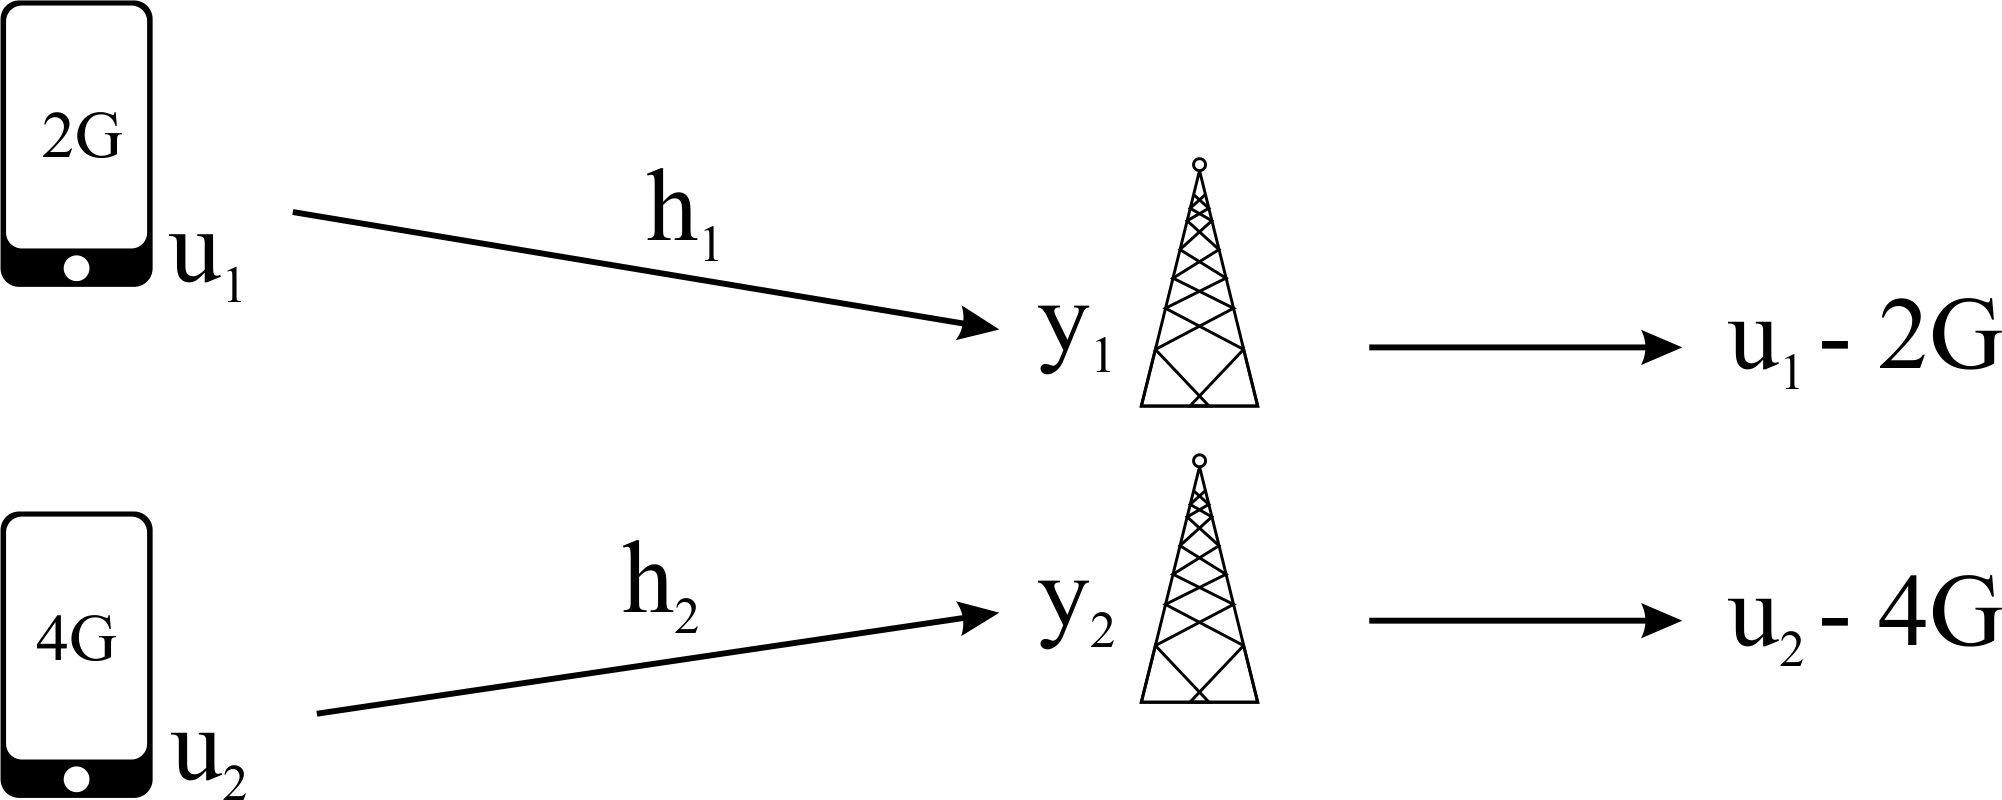
\includegraphics[scale=0.3]{pict/scheme2.jpg}
%\scriptsize Conventional Scheme
%\end{center}
%
%\begin{center}
%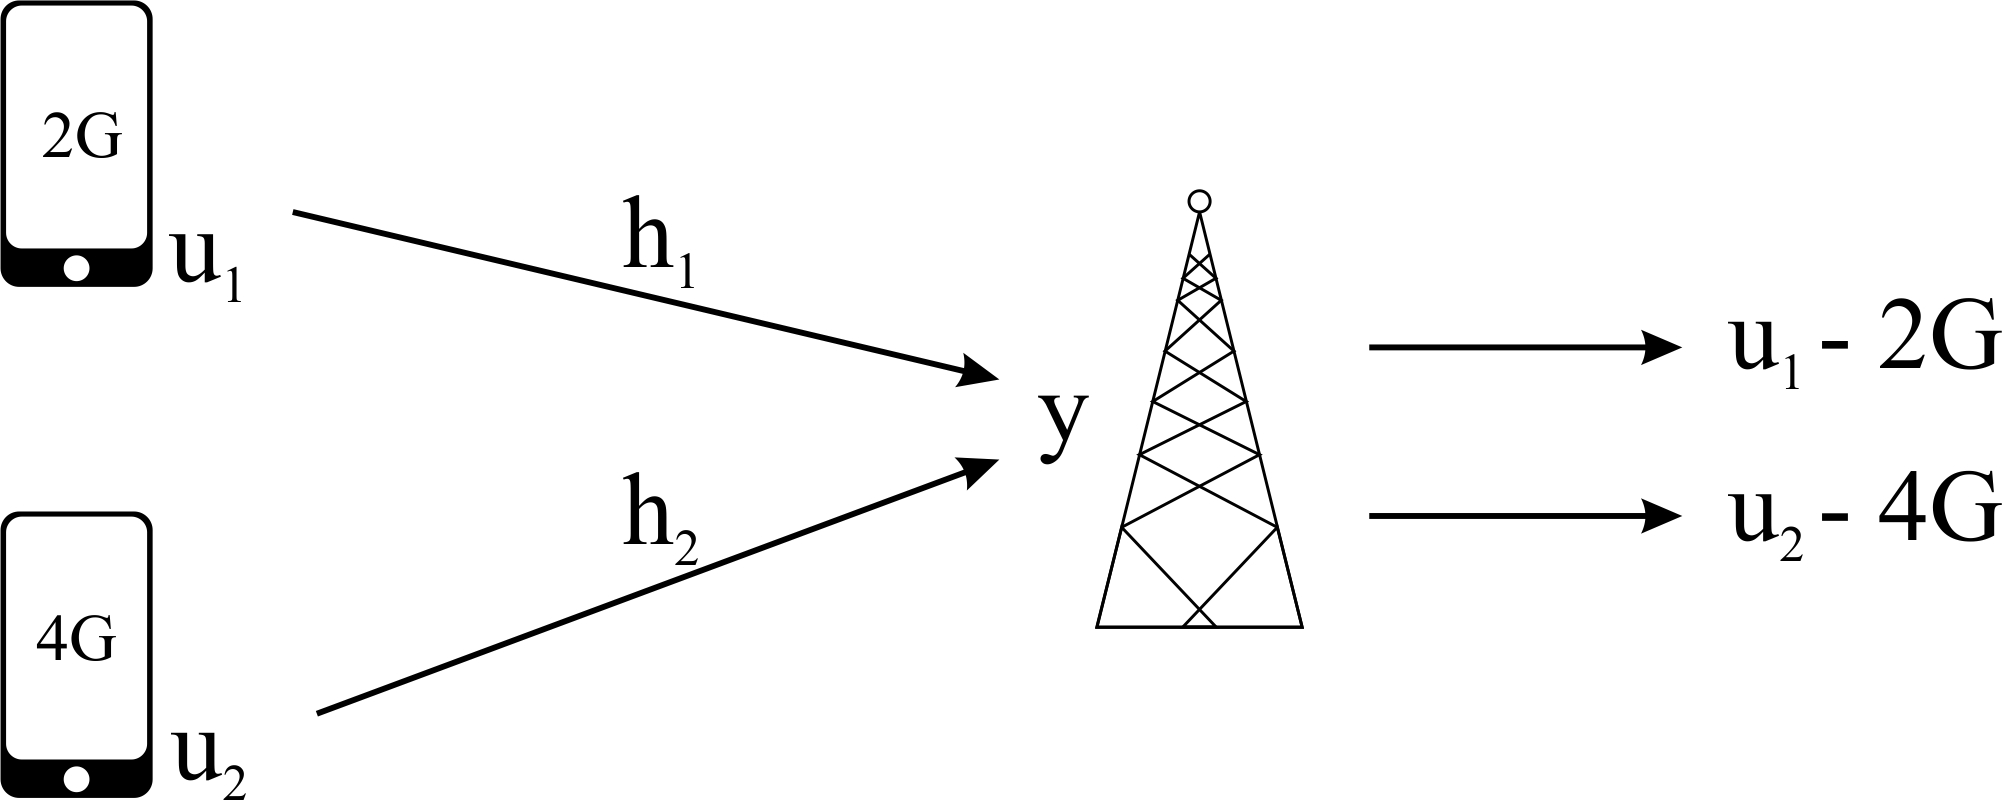
\includegraphics[scale=0.3]{pict/scheme1.jpg}
%\scriptsize Proposed Scheme
%\end{center}
%
%\column{0.5\textwidth}
%\begin{enumerate}\vspace{-0.2cm}
%\item \footnotesize {Conventional Scheme}
%\begin{itemize}
%\item[\textendash] \scriptsize {The signal detection based on generation frequency.}
%\item[\textendash] \scriptsize {Use more than 1 detection device.}
%\end{itemize}\vspace{0.2cm}
%\item \footnotesize{Purposed Scheme}
%\begin{itemize}
%\item[\textendash] \scriptsize{The signal detection using header on the package.}
%\item[\textendash] \scriptsize{Detect the user more accurate.}
%\end{itemize}
%\end{enumerate}
%\end{columns}
%\end{frame}

%\section{Theory}
%\begin{frame}
%\tableofcontents[currentsection,currentsubsection]
%\end{frame}
%--------------------------------------------------------------------------------------
\begin{frame}
\frametitle{Outlines}
\setbeamercolor{alert text}{fg=gray,bg=}
\begin{enumerate}
%\item Introduction
\item Motivation
\item \alert<+> {Basic Theories}
\item Research Trajectory
%\item Analysis
\item Conclusion 
\end{enumerate}
\end{frame}
\begin{frame}[shrink]{Basic Theory}
\framesubtitle{Introduction of Digital Video Broadcasting — Second Generation Terrestrial (DVB-T2)}
\begin{columns}[onlytextwidth]
\begin{column}{1\columnwidth}
\centering
\begin{itemize}\vspace{0cm}
\item \small DVB-T2 is a standard for digital terrestrial television broadcasting, offering significant benefits compared to  DVB-T both of it used Coded Orthogonal Frequency Division Multiplex (COFDM)\footnotemark[1]. 
\item \small Main benefit of the DVB-T2 over DVB-T is the possibility to increase the capacity in digital terrestrial television (DTT)\footnotemark[2].
\end{itemize}
\smallskip
\begin{center}
\begin{figure}
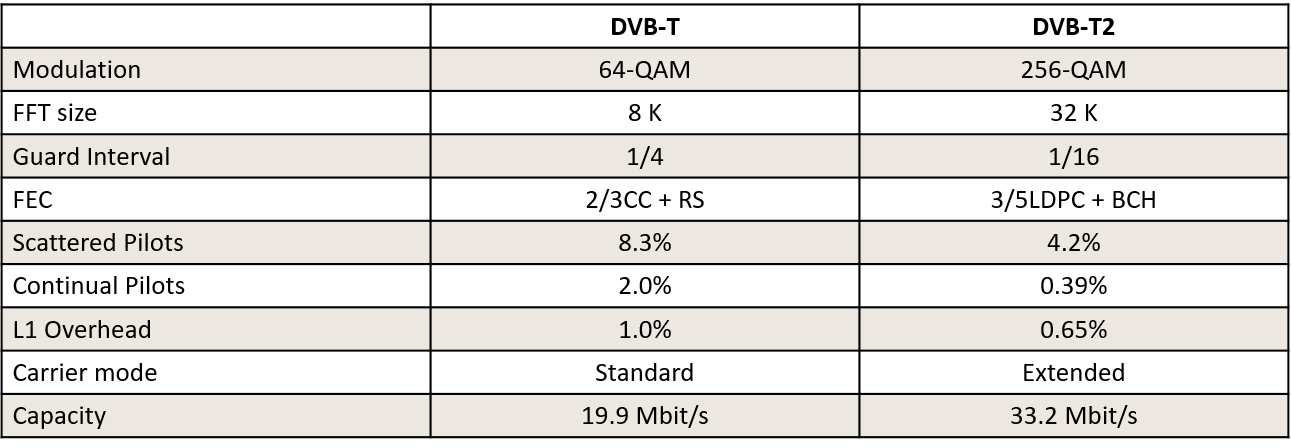
\includegraphics[scale=0.355]{pict/tabel.png}
\caption*{\tiny \centering The comparison between DVB-T2 and DVB-T for a long guard interval (SFN) mode, with the same absolute guard interval in both cases.}

\end{figure}
\end{center}
\end{column}
\end{columns}
\footnotetext[1]{\cite{etsi1}}
\footnotetext[2]{\cite{etsi2}}
%\begin{center}\vspace{0.6cm}\hspace{-0.5cm}
%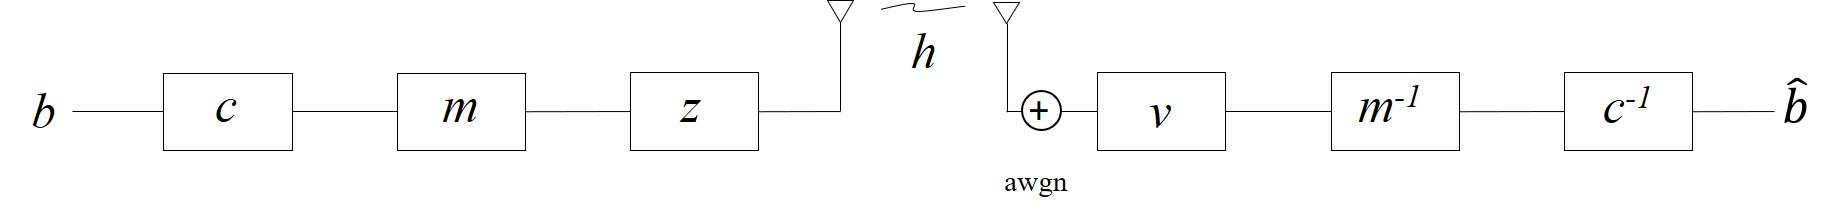
\includegraphics[scale=0.35]{pict/Header.jpg}
%\end{center}
%\vspace{0.7cm}
%\begin{columns}
%\hspace{1.5cm}
%\column{0.5\textwidth}
%\Large{}
%\scriptsize{\\ 
%\textit{b} = binary information\\
%\textit{c} = coded \textit{b}\\
%\textit{m} = modulation\\
%\textit{z} = adding header\\
%\textit{s} = adding syncronizer}
%
%\column{0.5\textwidth}
%\hspace{-2.3cm}
%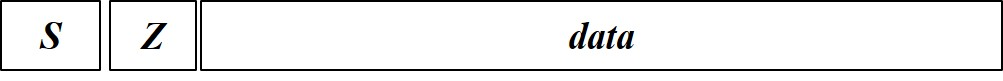
\includegraphics[scale=0.38]{pict/sync.jpg}
%\end{columns}
\end{frame}
\begin{frame}[shrink=23]{Basic Theory}
\framesubtitle{Low Density Parity Check (LDPC) Codes}
\begin{itemize}
\justifying
\item LDPC codes or sometimes called Gallager’s code were originally proposed in 1962 by Robert Gallager, One of error correction method have been proved to be capable of closely approaching the channel capacity \footnotemark[1].\\
\item LDPC codes of almost any rate and blocklength can be created simply by specifying the shape of the parity check matrix (H) \footnotemark[1].\\
\item Low-density parity-check codes are codes specified by a matrix containing mostly 0’s and only a small number of 1’s \footnotemark[2].\\

\item Parity check matrix H\\
\begin{itemize}
		\item[$\checkmark$] Long block length $n$\\
		\item[$\checkmark$] Variable node degree $d_v$\\
		\item[$\checkmark$] Check node degree $d_c$\\    		
\end{itemize}
\item[$\square$]Regular LDPC 	: \\
\begin{itemize}
			\item[$\checkmark$] $d_v=fixed$\\
     	  	\item[$\checkmark$] $d_c=fixed$\\
\end{itemize}
\item[$\square$]Irregular LDPC	: 
\begin{itemize}			
			\item[$\checkmark$] $d_v=not fixed$
     	  \item[$\checkmark$] $d_c=not fixed$
\end{itemize}
\end{itemize}
\begin{picture}(0,0)
\put(200,8){
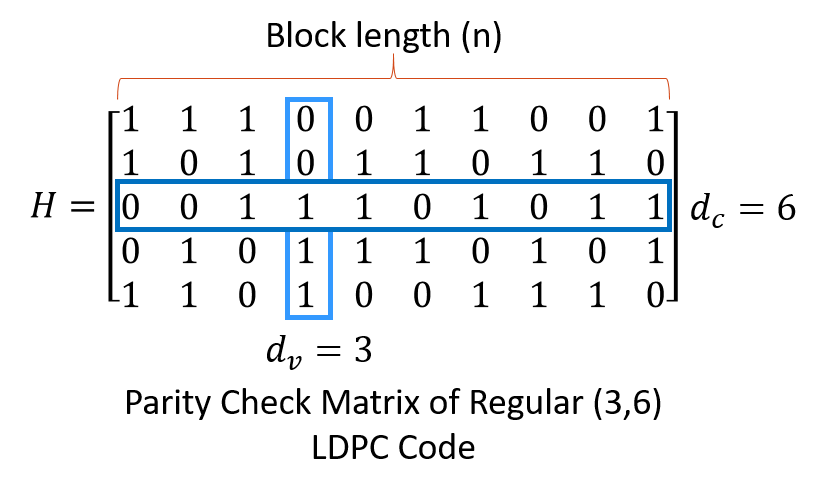
\includegraphics[scale=.6]{pict/matrice.png}}
%\caption*{\small \centering Parity Check Matrix of Regular (3,6) LDPC Code.}
\end{picture}
%Hadamard codes is codes with value $\pm $ 1 which can be formed into new matrix using Kronecker product. Hadamard codes matrix size $H(f)$ is $2^0{f}\times 2^{f}$
%\begin{center}
%\begin{eqnarray}
%H(f=1)&=&
%\begin{bmatrix}
% 1&1 \\ 
% 1&-1 
%\nonumber
%\end{bmatrix}\\
%H(f=i)&=&H(f=i-1)\otimes H(f=1)\nonumber\\ 
%H(f=2)&=&
%\begin{bmatrix}
%1&1&1&1\\
%1&-1&1&-1\\
%1&1&-1&-1\\
%1&-1&-1&1
%\nonumber
%\end{bmatrix}
%\end{eqnarray}
%\end{center}
\footnotetext[1]{\cite{koding1}}
\footnotetext[2]{\cite{ldpc6}}
\end{frame}

\begin{frame}[shrink=28]{Basic Theory}
\framesubtitle{Irregular Low-Density Parity-Check (LDPC) Codes}
\begin{itemize}
\justifying
	\item LDPC codes in DVB-T2 are irregular LDPC codes and the error-protection level of each code bit is not uniform, but depends on the column weight of the parity-check matrix \footnotemark[1].
	\item Irregular LDPC codes can substantially outperform similar codes based on regular LDPC codes \footnotemark[2].
	\item The irregular LDPC codes associated with the column $\lambda(x)$ and row distribution $\rho(x)$ :


%	\begin{columns}
%		\column{0.4\textwidth}
%		Cross Correlation is a value which indicate resemblance of two vector with multiply both of the vector and can be described with following equation.
%		\begin{equation}
%		R_{zz}=E[\hat{z}(t)\cdot\bar{z}(t-\tau)]
%		\nonumber
%		\end{equation}
%		with $\hat{z}$ is original header, $\bar{z}$ is received header, $E[\cdot]$ is expected value and $\tau$ is moving index.
%		\column{0.52\textwidth}
%		\begin{flushleft}\vspace{-0.2cm}
%			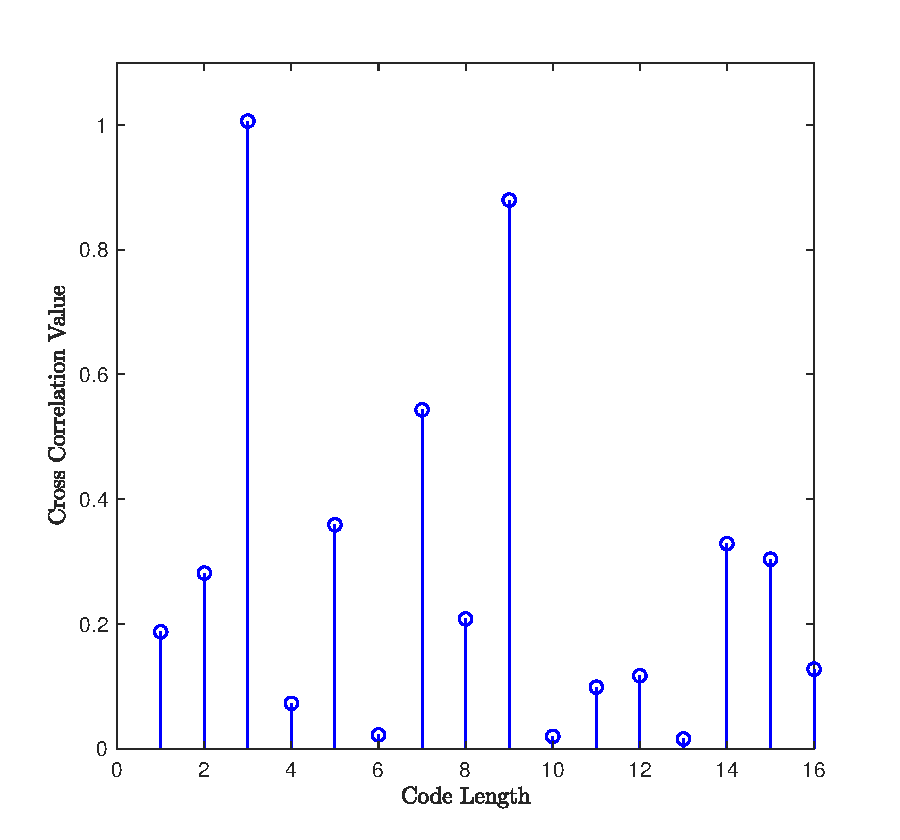
\includegraphics[width=2.8in]{pict/keluaran_cc}
%		\end{flushleft}
%	\end{columns}
\begin{block}{}
\begin{gather}
\lambda  (x)=\sum_{i= 2}^{dv}\lambda_{i}x^{i-1} \qquad  \rho (x)=\sum_{i= 2}^{dc}\rho_{i}x^{i-1}
\end{gather}
\end{block}
\item Example :
\begin{multicols}{2}

  \null \vfill
  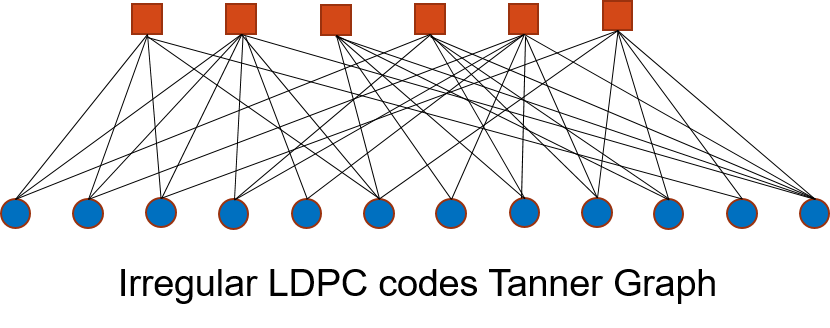
\includegraphics[scale=.5]{pict/irre.png}
  \vfill \null

\columnbreak

   \vfill
\justifying
So,\\
  \begin{gather}
 \rho (x)=\frac{1}{6}x^{4}+\frac{2}{6}x^{5}+\frac{1}{6}x^{6}+\frac{2}{6}x^{7} \\
 \lambda (x)=\frac{3}{12}x^{2}+\frac{7}{12}x^{3}+\frac{1}{12}x^{4}+\frac{1}{12}x^{5}
  \end{gather}
  \vfill \null
\end{multicols}

%\begin{picture}(0,0)
%\put(-60,-110){
%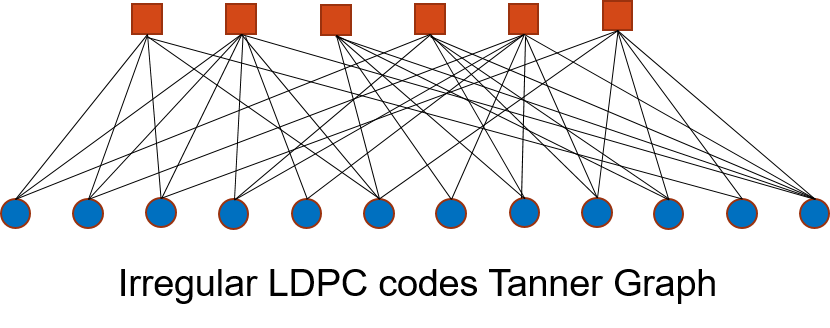
\includegraphics[scale=.6]{pict/irre.png}}
%\end{picture}
\end{itemize}
\footnotetext[1]{\cite{etsi1}}
\footnotetext[2]{\cite{ldpc7}}
\end{frame}

\begin{frame}[shrink=24]{Basic Theory}
\framesubtitle{DVB-T2 LDPC Standards}
\begin{itemize}
	\justifying
	\item LDPC codes in DVB-T2 are irregular LDPC codes and the error-protection level of each code bit is not uniform, but depends on the column weight of the parity-check matrix \footnotemark[1].
	\item The block length for LDPC code in DVB-T2 for normal codes $N_{ldpc}=64800$ and for the short codes $N_{ldpc}=16200$ [1].
	\item Standard code rate for DVB-T2 is $1/2, 3/5, 2/3 , 3/4, 4/5,$ and $5/6$.
	\item Cyclic structure used for implementation of encoder and decoder, Staircase structure used for generating parity bits by an accumulator.
	\item In DVB-T2, a bit interleaver having $Nc = 2m$ columns is used for the $2^{m}-QAM$ constellation - except for 256-QAM with the short code, which uses $m = 8$ columns.
\end{itemize}
\begin{picture}(0,0)
\put(40,-110){
\includegraphics[scale=.6]{pict/basic.png}}
%\caption*{\small \centering Parity Check Matrix of Regular (3,6) LDPC Code.}
\end{picture}
\footnotetext[1]{\cite{etsi1}}
\end{frame}

%\section{Simulation Result}
%\begin{frame}
%\tableofcontents[currentsection,currentsubsection]
%\end{frame}
%--------------------------------------------------------------------------------------


\begin{frame}[shrink=34]{Basic Theory}
\framesubtitle{EXIT Chart}
\begin{multicols}{2}

  \null \vfill
  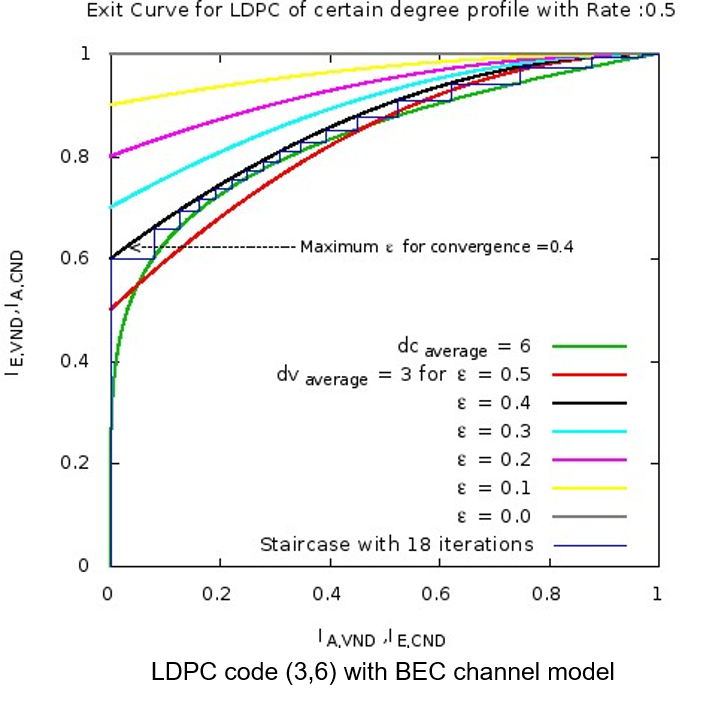
\includegraphics[scale=.6]{pict/lol.png}
  \vfill \null

\columnbreak

  \null \vfill
  \begin{itemize}
\justifying
\item \textbf{EX}trinsic \textbf{I}nformation \textbf{T}ransfer (EXIT) Chart introduced by Stephan ten Brink, it's a method used to evaluate performance of any iterative decoder and giving a feedback on required number of iterations to reach successful decoding\footnotemark[1].
\\
\item The chart is plotted as the a priori mutual information $I_A$ before message is decoded and the extrinsic mutual information $I_E$ after decoding.
\item EXIT charts can also be established for LDPC codes, the Variable Node decoder (VND) and the Check Node decoder (CND).
\item The output extrinsic mutual information of a variable node and check node denoted as $I_{E,VND}$ and $I_{E,CND}$, for the input a priori mutual information of a variable node and check node denoted as $I_{A,VND}$ and $I_{A,CND}$.
\end{itemize}
  
  \vfill \null
\end{multicols}

%\begin{columns}
%\column{0.33\textwidth}
%\column{0.33\textwidth}
%\hspace{0.7cm}
%\footnotesize{$y=$ Receive Signal,}\\
%\hspace{0.7cm}
%\footnotesize{$h=$ Channel,}\\
%\hspace{0.7cm}
%\footnotesize{$u=$ Transmit Signal}
%\column{0.33\textwidth}
%\end{columns}
\footnotetext[1]{\cite{exit1}}
\end{frame}

\begin{frame}
\frametitle{Outlines}
\setbeamercolor{alert text}{fg=gray,bg=}
\begin{enumerate}
%\item Introduction
\item Motivation
\item Basic Theory
\item \alert<+> {Research Trajectory}
%\item Analysis
\item Conclusion 
\end{enumerate}
\end{frame}
\begin{frame}{Research Trajectory}
\begin{center}
\begin{figure}\vspace{-2cm}\hspace{10cm}
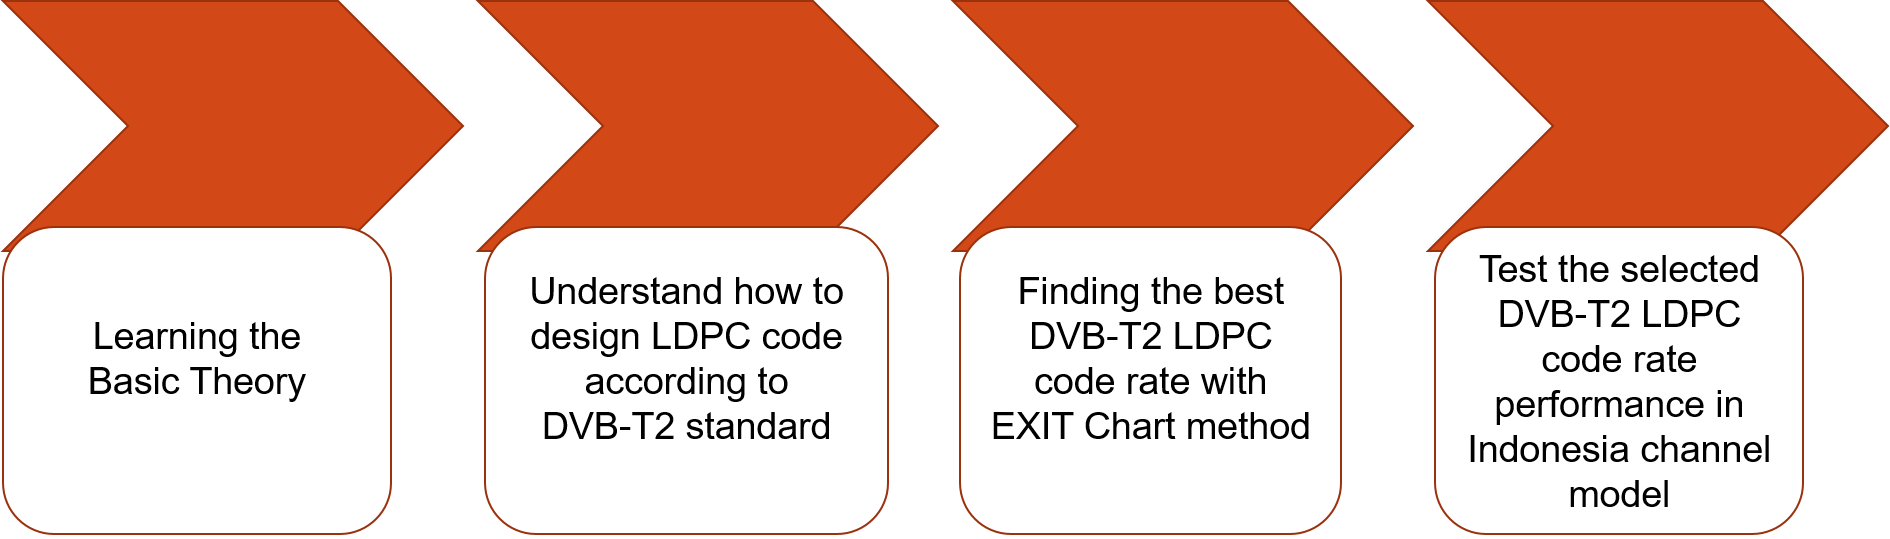
\includegraphics[scale=0.37]{pict/traject.png}
\caption*{\tiny Research Trajectory}
\end{figure}
\end{center}
\end{frame}

\begin{frame}
\frametitle{Outlines}
\setbeamercolor{alert text}{fg=gray,bg=}
\begin{enumerate}
%\item Introduction
\item Motivation
\item Basic Theory
\item Research Trajectory
%\item Analysis
\item \alert<+> {Conclusion} 
\end{enumerate}
\end{frame}
\begin{frame}{Conclusion}
This research will propose the rate of LDPC code for DVB-T2 in Indonesia channel model with the performance at BER, BLER, and outage probability using EXIT chart method. 

\end{frame}



%\begin{frame}{Simulation Result (Threshold)}
%\begin{itemize}
%\item MSE simulation Result of 2 Users using Threshold
%\begin{columns}
%\column{0.5\textwidth}
%\begin{center}\vspace{-0.5cm}
%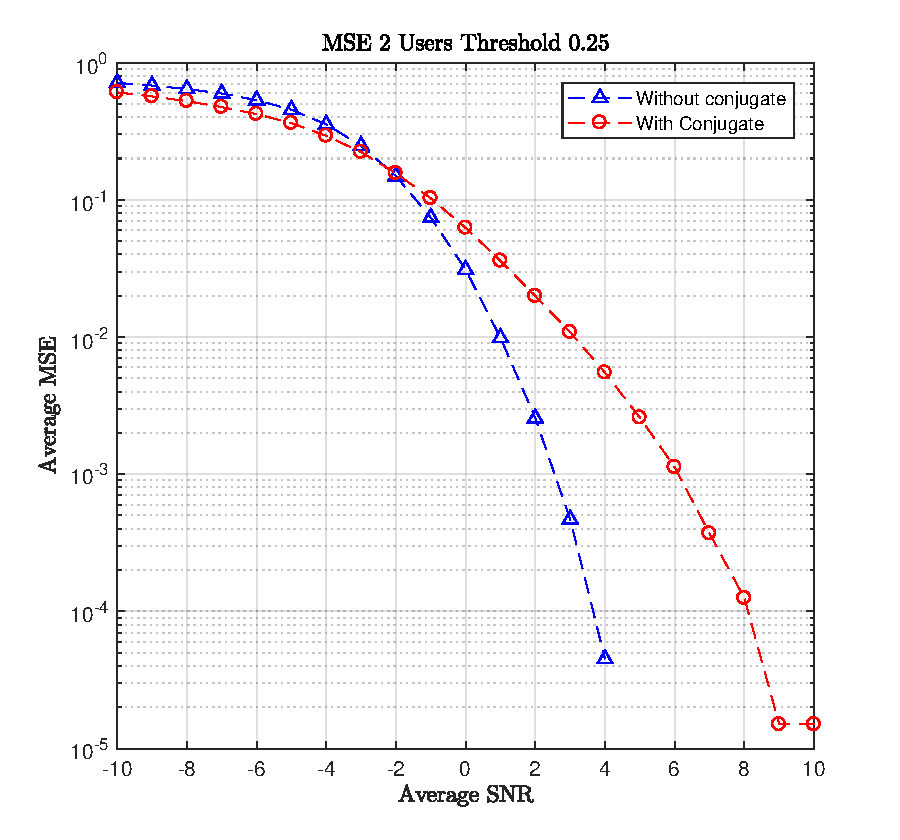
\includegraphics[scale=0.46]{pict/MSE_2user_alg1_alg2_th025.pdf}
%\end{center}
%\column{0.5\textwidth}
%\begin{center}
%\begin{itemize}
%\vspace{-2cm}
%\item[\textendash] \scriptsize{Threshold value $=$ 0.25.}
%\item[\textendash] \scriptsize{Header detection using threshold can obtain MSE without conjugate value less than with conjugate.}
%\item[\textendash] \scriptsize{Threshold is used for limiting cross correlation value.}
%\item[\textendash] \scriptsize{Cross correlation value less then threshold will be assume as loss signal caused by fading.}
%\end{itemize}
%\end{center}
%\end{columns}
%\end{itemize}
%\end{frame}

%\begin{frame}{Simulation Result}
%\begin{itemize}
%\item Comparison MSE
%\begin{columns}
%\column{0.5\textwidth}
%\begin{center}\vspace{-0.5cm}
%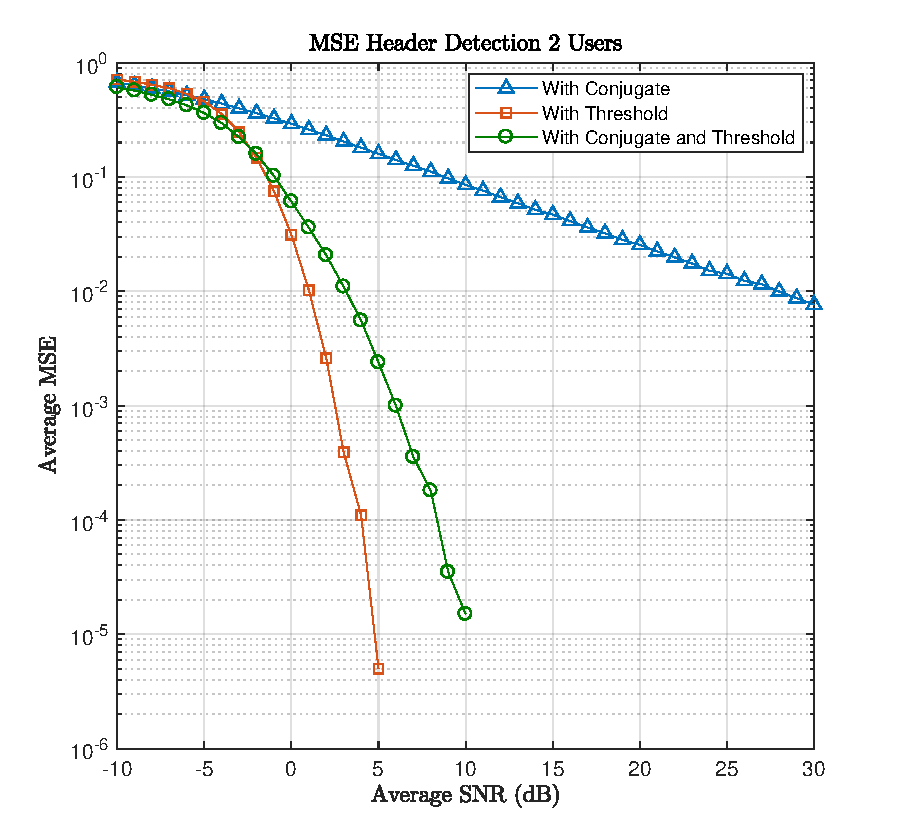
\includegraphics[scale=0.46]{pict/MSE_2user_alg1_alg2_banding.pdf}
%\end{center}
%\column{0.5\textwidth}
%\begin{center}
%\begin{itemize}
%\vspace{-1.5cm}
%\item[\textendash] \scriptsize{Header detection using threshold without conjugate value is lowest.}
%\end{itemize}
%\end{center}
%\end{columns}
%\end{itemize}
%\end{frame}
%
%\section{Conclusion and Next Homework}
%\begin{frame}
%\tableofcontents[currentsection,currentsubsection]
%\end{frame}
%--------------------------------------------------------------------------------------
%\begin{frame}{Conclusion and Next Homework}
%\vspace{-2cm}
%\begin{itemize}
%\item \footnotesize{Conclusion}
%\begin{itemize}
%\item[\textendash] \scriptsize{An equalizer used on the detection can reduce detection fault.}
%\item[\textendash] \scriptsize{Equalizer on this simulation can cancel the interference more accurate when the user number increase.}
%\end{itemize}
%\item \footnotesize{Next Homework}
%\begin{itemize}
%\item[\textendash] \scriptsize{Detection should detect user and device generation.}
%\end{itemize}
%\end{itemize}
%\end{frame}

\begin{frame}
\centering
\LARGE{Thank you}
\end{frame}
\end{document}
